\documentclass[letterpaper,10pt]{article}
\usepackage[margin=0.75in]{geometry}
\usepackage{graphicx}

\title{Not Exactly the Internet of Things for Outdoor Lighting:\\Progress Report}
\author{Oregon State University CS Senior Capstone Group 22\\Malcolm Diller, Sean Rettig, Evan Steele\\Client: Victor Hsu}
\date{\today, Fall Term}

\begin{document}

\maketitle

\section{Abstract}

Our group has made serious progress in the project to turn the Raspberry Pi and
ESP8266 Wifi module into a "Not exactly IoT" device for controlling 
binary devices wirelessly. From project assignment to week five, our group
produced a proof-of-concept for the final project, and planning the final
software approach in the meantime. Despite all the writing requirements this 
term, we made excellent progress.\\
Throughout the term, our team moved between early prototyping and detailed 
documentation for the project. With regular communication through email and IRC
our group kept coordinated throughout the term, publishing progress reports to
the Sharepoint site and code samples to our Github page. We will discuss our 
weekly progress and describe how the prototype and documentation unfolded over the 
course of the first term of the capstone project. This should provide an assessment
on where our groups stands in preparedness to move forward with implementation next term.

\pagebreak

\section{Progress}

% sean
\subsection{Week 3}

Our first week of the capstone project ``Not exactly the Internet of Things for
Outdoor Lighting'' was relatively uneventful, as we spent most of the time
coordinating group meetings.  At our first group meeting, we brainstormed a
list of clarifying questions to ask our client, Victor, about the project,
including:

\begin{itemize}
    \item How is the system going to be controlled by phones?  Is a dedicated
        app necessary, or can we provide a mobile-friendly website?\\ Answer: A
        mobile-friendly website is acceptable.
    \item Are we just going to be controlling lights, or are we going to expand
        to other devices if we have time (e.g. sprinkler system, music players,
        garage door openers, alarm systems)?\\
        Answer: The control of other devices is currently outside the scope of
        this project, but can be a stretch goal.
    \item Will the code for this project be open source?\\
        Answer: Yes!  The entire project is hosted on Github.com in a public
        repository.
    \item What hardware will we have access to?\\
        Answer: In addition to the hardware mentioned in the client's original
        project proposal, Victor agreed to order a 2.8" TFT Display with
        Resistive Touchscreen <http://www.adafruit.com/products/1774> for use
        with the Raspberry Pi in the control unit.
\end{itemize}

In addition, we were able to finish our Problem Statement document, which
largely involved expanding upon our client's original project proposal with
additional clarification, focus, technical details, and performance metrics.

% sean
\subsection{Week 4}
 
Progress since last week: 
We have started on our requirements document and listed the required and optional requirements. 
Problems: 
No problems this week. 
Plans for the coming week: 
Meet with our client to review our draft of the requirements document and finalize it. 
Start to work with the hardware as soon as we get it. This will probably consist of booting the Raspberry Pi with an operating system and compiling MicroPython on the Wifi Modules. 
If we get far enough, work on communication between the Pi and the controllers. 

\subsection{Week 5}

This week we completed our requirements document and began researching
the hardware once we had it in our hands. We picked up the Raspberry Pi
and TFTLCD display from Victor and booted the device with the \textit{fbtft} 
module for the device. This week was otherwise uneventful with everyone working
on other projects and midterms, but there was still work done with regards to 
group logistics and future planning. When we aren't so busy next week, we will
continue our proof of concept project to get the firmware and relay online.

% Malcolm
\subsection{Week 6}
 
Most of what we did on week 6 of our project involved trying to get a functioning proof of concept for our project, which turned out to be filled with more problems than anticipated. We began to investigate software packages and technologies that would help us meet the requirements outlined on our document. The main problem that we ran into this wee was with the wireless networking that we were planning on for the Pi.

We tested the devices with various wireless networking methods including ad-hoc and in access-point mode. While testing, we discovered that the ad-hoc system was not working as expected. This was due to the USB WiFi adapters we were using not being compatible with an ad-hoc setup. This was especially problematic because our main plan was to use ad-hoc for networking. After further investigation, it became clear that we would have to reevaluate our network implementation, as there would be no way to work around the issue and still use ad-hoc. We are now just using the Pi as a wireless access point. This solves the problems caused by the compatibility issues with ad-hoc.

In addition to working on the proof of concept, we also made headway on some of the documents that we had due soon. As we continued to develop the Technical Requirements document, we asked the TA to see if he had any comments on it. His advice was to elaborate more on the requirements we already had and make them as specific as possible. Following his advice, we expanded on our current requirements by adding more detail and specifying exactly what we meant. We also refined our elevator pitch to make it a better fit for the intended audience.

% Evan
\subsection{Week 7}  

After much delay, sweat and tears, we finally have a functional proof 
of concept to demo and show off. The program is super simple but 
accomplishes the bare minimum of what we would expect the program to do.
Sending a basic TCP command to the ESP8266 module will cycle the lights 
through the device's Lua firmware, and will in turn flip the relays out of
the board's GPIO once we wire it up too. The TCP commands are sent by the 
Raspberry Pi using a boot script on lxTerminal, using an execution sequence
that looks like this:
\begin{enumerate}
\item{Pi boots into the TFTLCD module, screen initialized}
\item{Pi loads lxTerminal, runs startup script in init.d}
\item{inid.d script connects to the ESP8266 module, gets an IP}
\item{After the connection is made, the inid.d script starts a Python script}
\item{The Python script cycles through TCP commands and send them to the device}
\end{enumerate}

For our next step, we need to make sure that the Pi can reliably perform
the discovery operation (the IP is hard-coded right now) and that the ESP8266
module can run as a client in the future, connecting to the Pi to take 
advantage of the Pi's DHCP server and to simplify future connections.\\

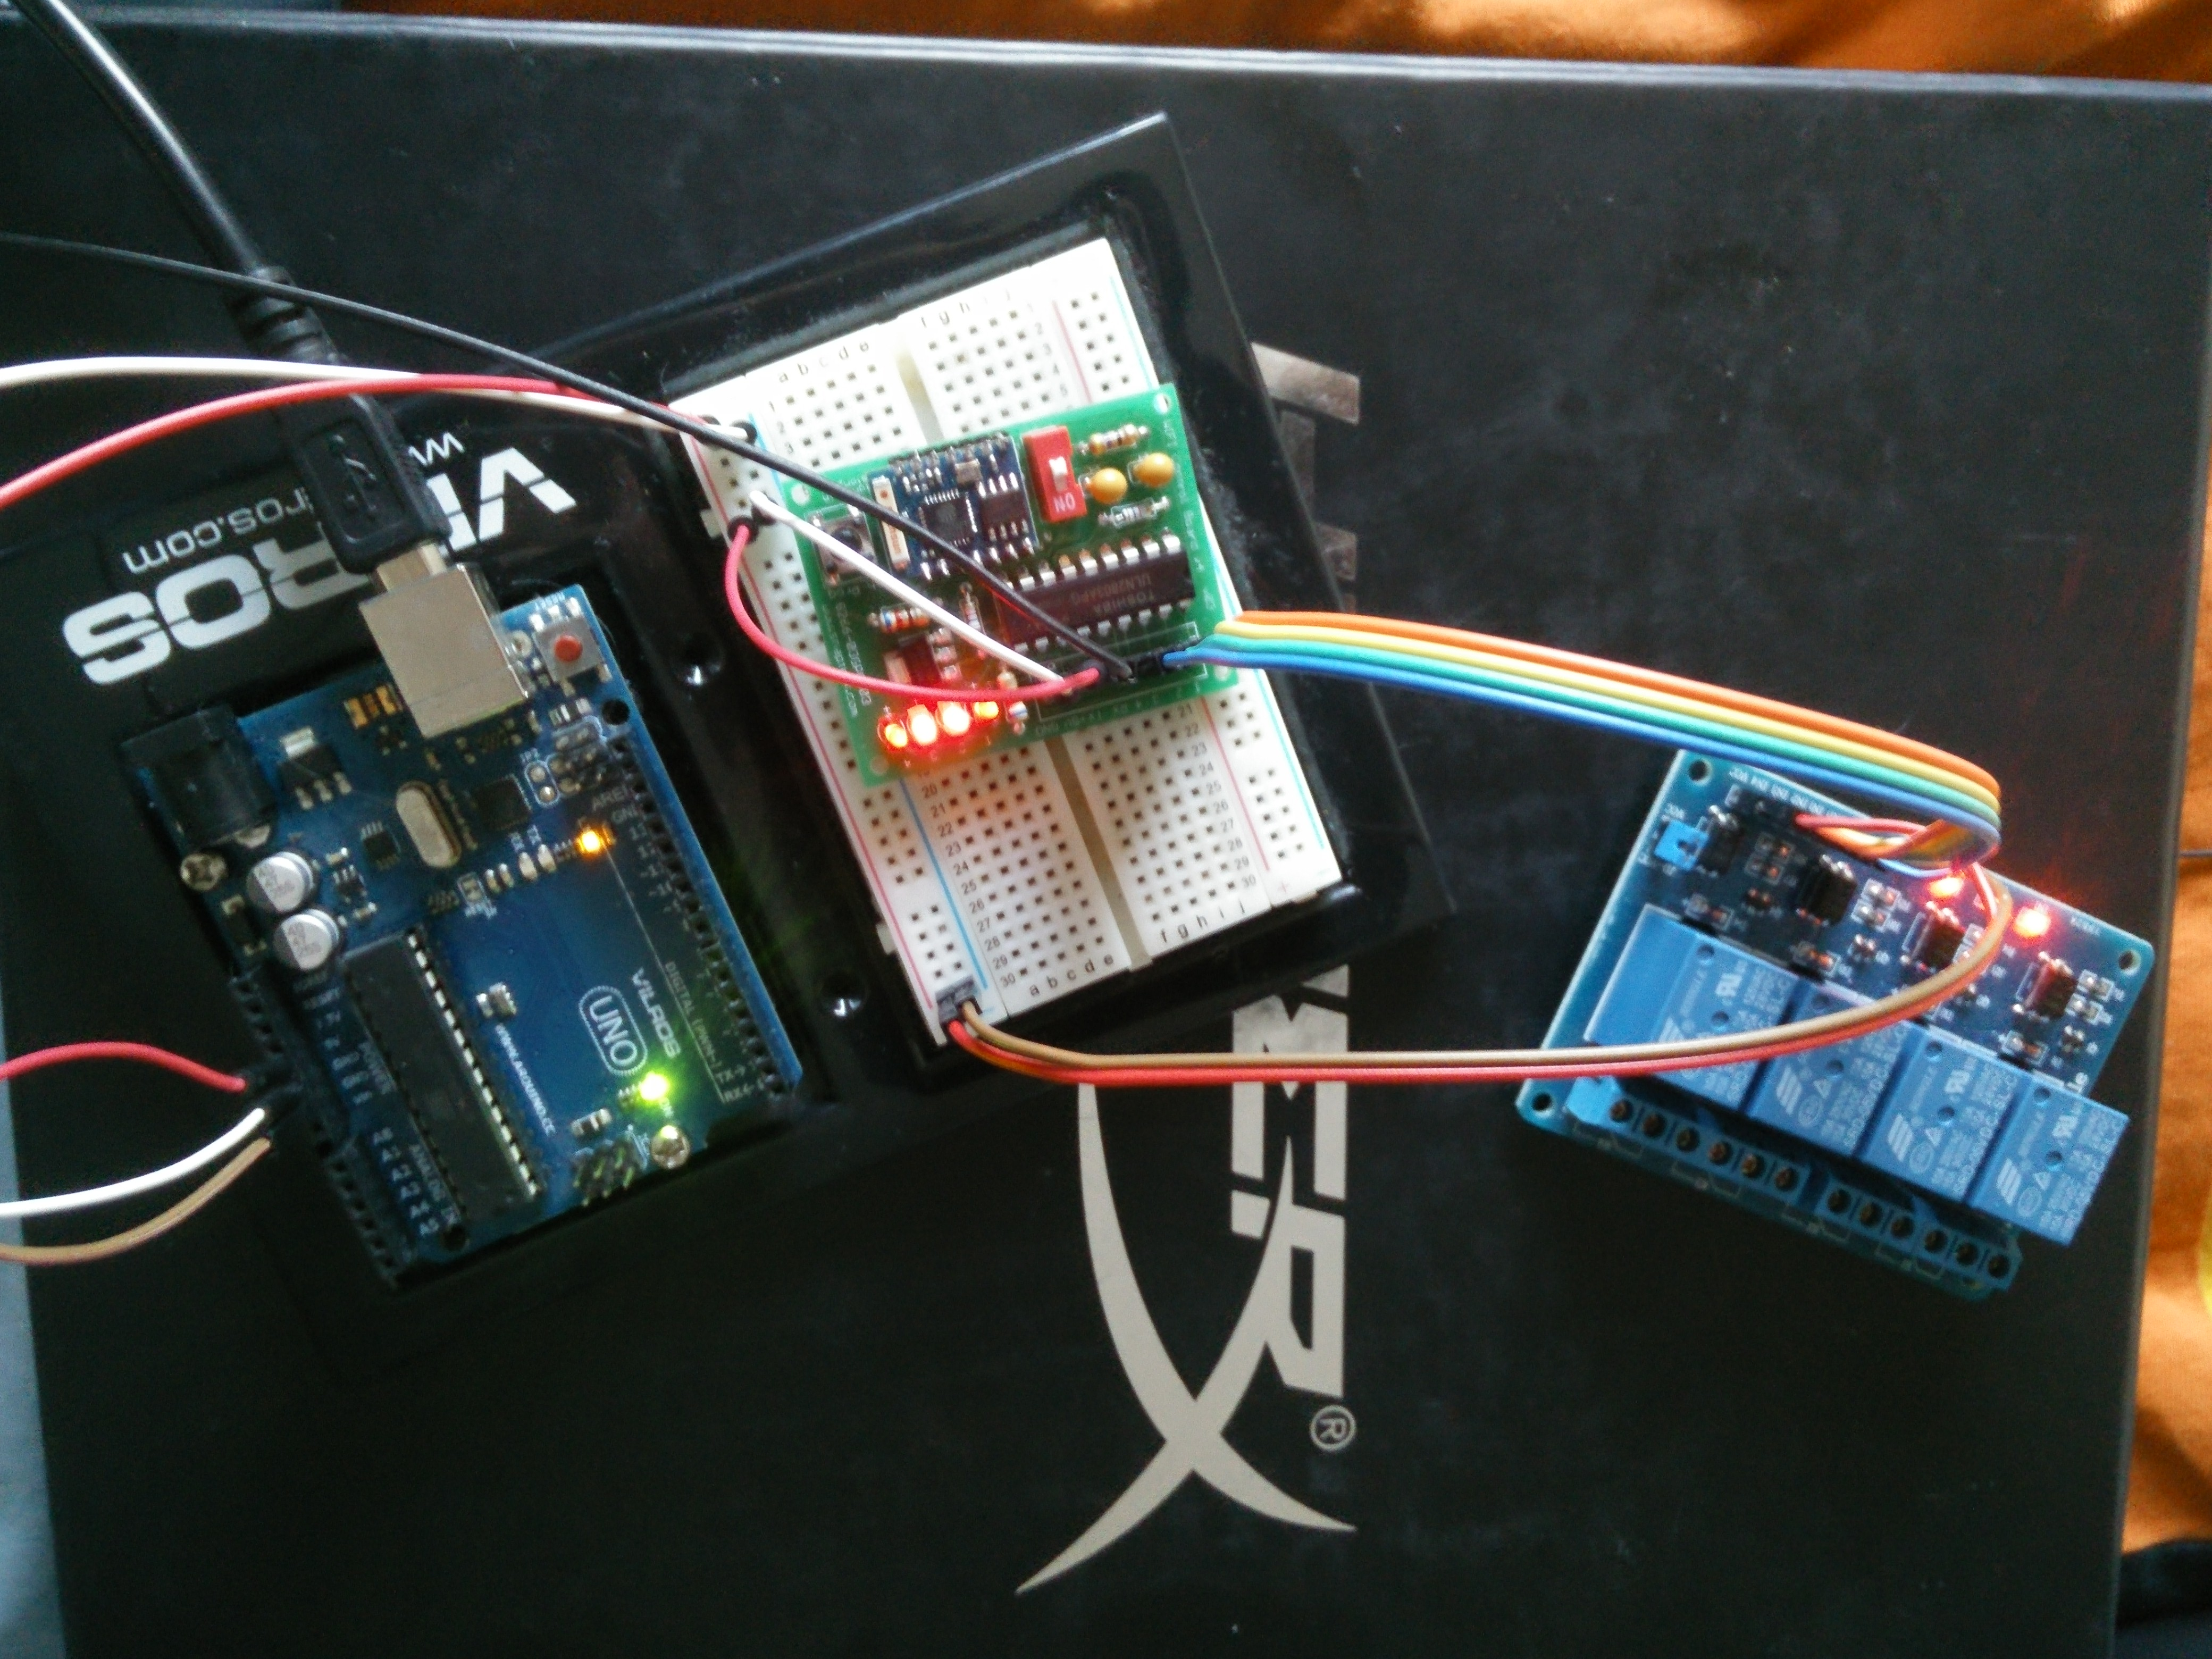
\includegraphics[scale=0.1]{circuit.jpg}

% sean
% Evan
\subsection{Week 8}
 
Progress since last week: 
 
Our proof of concept is now portable, and booting the pi connects it to the esp and cycles the lights on the relay. It has also been shown to the TA. 
Completed the expo poster 
Re-Wrote the elevator pitch 
Problems: 
No real problems this week 
Plans for next week: 
Continue to develop the proof of concept, possibly by adding actual lights to the relay instead of the LED's. 
Present the elevator pitch 

% Malcolm
\subsection{Week 9}
 
On Week 9 we continued to work on testing out our proof of concept. We managed to connect actual lights to our relay and verified that we can control them by toggling them on and off. This is a good step toward getting a fully working proof of concept working as it means we have most of the main parts done, and mainly need to start working on the UI of the touchscreen and web page.

We decided that we are most likely going to use Flask to implement the website. Flask is a micro-framework for Python that is designed for developing websites. The main reason we are planning on using it is that we are using Python for many of the other parts of the project, and so it would be easy to integrate this and also would make sense in terms of keeping the code consistent. To prepare for when we are ready to start implementing that, we have begun learning more about how Flask works, and how we might be able to use it to create our our website.

We also presented our elevator pitch on this week, which went decently well. There were no documents to turn in this week, and there was only class on Tuesday so there is not much else to report. Next week we planned to iron out the design document and work on the progress report. 

% Evan
\subsection{Week 10}
The final week of the capstone project was largely uneventful as our group began working on other final projects 
and studying for exams. However, we did get some work in with regards to some project details and the work on the design document. 
This week we took our document to the TA to get some feedback regarding the design elements we focused on for the paper, 
and he was pleased with the overall result after some vocabulary changes. 
The hardware project itself didn't get much direct attention this week, but we did wonder about the usability of the final result, from a user perspective. 
How easy-to-use should set-up be? Should the user have to worry about port forwarding on the home network? 
According to Victor, our project sponsor, there was no need to design an overly-simplified option. 
We will continue to investigate more networking options over break.

\begin{itemize}
    \item Completed: Design Document\\
	The design document was reviewed by our group and a TA and turned in. 
	we also had our weekly meeting with the TA at this time.  
    \item How complicated does the user-setup portion of the project need
	to be and are there restrictions on what they should be able to do?\\
        Answer: As of now, having to reconnect to the device to reconfigure 
	it is acceptable. Victor imagines that we won't have to connect so
	often that investing time into developing a complex networking option
	is not necessary.
    \item What will the project do over break?\\
        Answer: Evan will be taking the hardware home to use in his network
	testing bench, which is pretty much just a dozen microcomputers 
	plugged into an old Cisco 2960x networking together. 
\end{itemize}

Over break, Evan will be experimenting with some networking strategies and
working with the web serve to flip the relay. Sean suggested that Flask would
provide a good framework, but as of now he's the only one with experience in 
it, so Malcom and Evan will need to study it. An ideal goal for the start of 
Winter term would be having a working web interface that can flip the relay,
built with the Yocto build server. Even better if we have the interface
up on the TFTLCD screen, but we may save that until we get back together.

\end{document}
